\documentclass{article}
\usepackage[utf8]{inputenc}
\usepackage{amsmath}
\usepackage{amsfonts}
\usepackage{cite} 
\usepackage{breqn}
\usepackage{graphicx}
\usepackage{hyperref}

\allowdisplaybreaks

%Useful definitions
\providecommand{\Rie}[3]{\mathcal{R}_{#1}{}^{ #2}{}_{#3}}
\providecommand{\ctG}[3]{\Gamma_{#1}{}^{ #2}{}_{#3}}
\providecommand{\ctg}[3]{\gamma_{#1}{}^{ #2}{}_{#3}}
\providecommand{\B}[3]{\mathcal{B}_{#1}{}^{ #2}{}_{#3}}
\providecommand{\P}[3]{\mathcal{P}_{#1}{}^{ #2}{}_{#3}}
\providecommand{\A}[1]{\mathcal{A}_{#1}}
\providecommand{\Ri}[1]{\mathcal{R}_{#1}}
\providecommand{\deV}[1]{\mathrm{d}V^{#1}}


\title{Cosmological solutions with torsion effects in Polynomial Affine Gravity}
\author{Jos\'e Perdiguero G\'arate}

\begin{document}

\maketitle
%\tableofcontents

\section{Introduction}
\label{sec:Introduction}

Einstein's theory of General Relativity, it is a gravitational theory where the interaction is solely mediated by the 
metric tensor \cite{Einstein_GR,Einstein_GR_Bases}. Providing an ansatz compatible 
with the symmetries of the observable universe (cosmological principle), it is possible to model the Universe with Einstein's
field equations \cite{Einstein_GR_Feqs}.

With the introduction of the cosmological constant (see Ref. \cite{Einstein_Cosmological_Constant}) it is possible to obtain nontrivial dynamics to 
describe the evolution of the universe, leading to nine different scenarios, depending on the values of the geometrical factor $\kappa$ (which characterize
the geometry of the spatial foliation of the Universe), and the cosmological constant $\Lambda$. Although, the introduction of a 
cosmological constant does indeed introduce a repulsive force required to keep the universe in static equilibrium, this idea 
does not provide a precise description of the current state of the universe. In order to have a more accurate description of the observable universe,
it is required the introduction of the energy-momentum tensor, along with the state equation. By taking into account this new information into 
Einstein's Field Equations, it is possible to portray the observable universe. Moreover, it allow us to clearly distinguish three different 
epochs, \textit{evolving} from a radiation era, to a matter era and finally to an accelerated expansion due to dark energy presence. This is the 
universe describe by Friedmann–Lemaitre–Robertson–Walker (FLRW), see Refs. \cite{Frie,Friedmann,Lema,Lema_Expansion,Robertson_1,Robertson_2,Robertson_3}, 
and provides the foundations for the standard model of cosmology $\Lambda$CDM.

Einstein's formulation its the best theory we have so far to describe gravitational interactions, and there is an agreement between the theoretical
predictions with the observational data, to see a full review on its empirical evidence, see Ref. \cite{Will_2014,will_2018}. Perhaps, one of its more
important theoretical predictions, it is the existence of gravitational waves, which were detected by by LIGO-Virgo collaborations \cite{Abbott_2016,Abbott_2017}.
Despite its success, there are still nontrivial problems related to its description of the geometry of space-time, specifically problems related 
to a quantization of gravity \cite{PhysRev.160.1113,PhysRev.162.1195,PhysRevD.10.401,PhysRevD.10.411} and 
the necessity of the dark sector to explain the galaxy rotation curve speed \cite{Rotation_Curve,Rotation_Curve_2}, along with accelerated expansion \cite{Riess_1998}.

These type of problems suggest, in principle, Einstein's theory of gravity must be an effective theory of another gravitational theory. In that sense, 
there are extensions of general relativity such as where the Einstein-Hillbert action its replaced by an arbitrary function, named $f(\mathcal{R})$, 
which was first proposed in Ref. \cite{10.1093/mnras/150.1.1}. An interesting case of this type of gravity, its the Starobinsky's model \cite{STAROBINSKY198099} 
that allows to describe a universe without a singularity. Moreover, due to quantum corrections to general relativity, lead to a new contribution 
to the Einstein-Hillbert action due to curvature squared new term \cite{1979ZhPmR..30..719S}, which is a special case of $f(\mathcal{R})$ gravity. 

Because the choice on function $f(\mathcal{R})$ it is an arbitrary one, there is an abundance of cosmological models, however, one could go even 
further and at a fundamental level, claim, that the metric tensor and the affine connection (a prior) must be independent fields, these are 
the type of modify models are known as \textit{metric-affine} models, and its formalism it is known as \textit{Palatini} formalism. There is an 
extensive collection on the literature related to metric-affine models \cite{Hehl_1995,Baldazzi_2022,Vitagliano_2011,Karahan_2012,SARDANASHVILY_2011}, and 
an extensive/complete review can be found in Ref.\cite{OLMO_2011}.

In addition, its possible to built models of gravity with the affine connection as its fundamental field. The first affine model of gravity was proposed by
Sir Eddington \cite{Eddington1923-EDDTMT}, and pure affine formalism were proposed in Refs. \cite{Krasnov_2011,poplawski2007unified,POP_AWSKI_2007}. 
These type of affine formulations models of gravity, use the square-root of the Ricci tensor instead of the metric tensor to define the invariant volume element

There are other extensions to Einstein's theory of general relativity, for example Einstein-Cartan model \cite{ASENS_1924_3_41__1_0,ASENS_1925_3_42__17_0}, 
which uses the Einstein-Hillbert action to define gravitational interactions, with a non-symmetric connection by introducing nontrivial 
torsion effects. Moreover, the inclusion of extra dimensions where first proposed and studied by T. Kaluza and O. 
Klein in Refs. \cite{Kaluza_Klein}, specifically, uses a fifth dimension which allows to unify the gravitational with an 
electromagnetism forces. There are many gravitational models and within different classifications, an illustrative example 
of a so-called \textit{map of modify gravity} can be found in Ref. \cite{Shankaranarayanan_2022}.

In order to built a purely affine gravitational model of gravity, the metric tensor can not play any role in its formulation and in its building blocks, and this is
where the Polynomial Affine Gravity enters. The Polynomial Affine Gravity its an alternative and purely affine model of gravity whose fundamental field is the affine connection instead
of the metric tensor. The model has been studied in Refs.\cite{castillofelisola2016polynomial,castillofelisola2016einsteins,castillofelisola2019cosmological,
Castillo_Felisola_2018,Castillo_Felisola_2020,Castillo_Felisola_2022_EPJC,Castillo_Felisola_2022_Universe} and on this work, we explore the
consequences of including torsion effects in its field equations in four-dimensions.

This paper is organized as follows: In Section \ref{sec:PAG}, we present a brief overview on how to built the Polynomial Affine Gravity model, highlighting
its features, and how it is possible to still have two different emergent-metrics structures despite being a purely affine model. A complete scan of cosmological
solutions to the field equations is presented in Section \ref{sec:solutions}. In Section \ref{sec:analysis}, we analyse and discuss the cosmological 
solutions. Final remarks are presented in Section \ref{sec:final_remarks}. 

\section{Polynomial Affine Gravity}
\label{sec:PAG}

The Polynomial Affine Gravity is a model of gravity whose fundamental field is the affine connection $\hat{\Gamma}$,\footnote{The action is polynomial
in the connection and its derivative} whose irreducible fields can be decomposed into its symmetric and skew symmetric part
\begin{equation}
\begin{aligned}
    \label{affine_connection}
    \hat{\Gamma}_{\alpha}{}^{\beta}{}_{\gamma} & = \hat{\Gamma}_{(\alpha}{}^{\beta}{}_{\gamma)} +  \hat{\Gamma}_{[\alpha}{}^{\beta}{}_{\gamma]},  \\
    & = \ctG{\alpha}{\beta}{\gamma} + \B{\alpha}{\beta}{\gamma} + \delta^{\beta}_{[\gamma}\A{\alpha]},
\end{aligned}
\end{equation}
the first term corresponds to the symmetric part of the connection $\hat{\Gamma}_{(\alpha}{}^{\beta}{}_{\gamma)} = \ctG{\alpha}{\beta}{\gamma}$, whereas
the last two terms are related to the torsion tensor, the former traceless component of the torsion $\B{\alpha}{\beta}{\gamma}$ and the latter corresponds 
to its vectorial part $\A{\alpha}$.

Since the symmetric part of the connection does not preserve the invariance under diffeomorphisms, it enters into 
the action through the covariant derivative $\nabla^{\Gamma}$. Additionally, the volume form is defined by the wedge product (which does not
required the metric tensor to be well-defined) $\deV{\alpha\beta\gamma\delta} = \mathrm{d}x^{\alpha}\wedge\mathrm{d}x^{\beta}\wedge
\mathrm{d}x^{\gamma}\wedge\mathrm{d}x^{\delta}$.

Therefore, the fundamental building blocks in our affine model of gravity are $\nabla$, $\mathcal{B}$, $\mathcal{A}$ and $\mathrm{d}V$. The action is built up using
a sort of \textit{dimensional analysis} technique. The method allows us to consider every scalar densities composed by powers
of the irreducible fields of the affine connection \cite{castillofelisola2016einsteins,Castillo_Felisola_2020}. In the same spirit the three-dimensional model was also built up Ref. \cite{Castillo_Felisola_2022_EPJC}.

The most general action (up to topological invariants and boundary terms) in four dimensions is given by
\begin{equation}
    \label{PAG_action}
    \begin{split}
    S
    & =
    \int  \mathrm{d}V^{\alpha \beta \gamma \delta} \bigg[
    B_1 \mathcal{R}_{\mu\nu}{}^{\mu}{}_{\rho}\mathcal{B}_{\alpha}{}^{\nu}{}_{\beta}\mathcal{B}_{\gamma}{}^{\rho}{}_{\delta}
    + B_2 \mathcal{R}_{\alpha\beta}{}^{\mu}{}_{\rho} \mathcal{B}_{\gamma}{}^{\nu}{}_{\delta} \mathcal{B}_{\mu}{}^{\rho}{}_{\nu}
    + B_3 \mathcal{R}_{\mu\nu}{}^{\mu}{}_{\alpha} \mathcal{B}_{\beta}{}^{\nu}{}_{\gamma} \mathcal{A}_\delta
    \\
    & \quad
    + B_4 \mathcal{R}_{\alpha\beta}{}^{\sigma}{}_{\rho}\mathcal{B}_{\gamma}{}^{\rho}{}_{\delta}\mathcal{A}_\sigma
    + B_5 \mathcal{R}_{\alpha \beta}{}^{\rho}{}_{\rho} \mathcal{B}_{\gamma}{}^{\sigma}{}_{\delta} \mathcal{A}_\sigma
    + C_1 \mathcal{R}_{\mu\alpha}{}^{\mu}{}_{\nu} \nabla_\beta \mathcal{B}_{\gamma}{}^{\nu}{}_{\delta}
    \\
    & \quad
    + C_2 \mathcal{R}_{\alpha\beta}{}^{\rho}{}_{\rho} \nabla_\sigma \mathcal{B}_{\gamma}{}^{\sigma}{}_{\delta}
    + D_1 \mathcal{B}_{\nu}{}^{\mu}{}_{\lambda} \mathcal{B}_{\mu}{}^{\nu}{}_{\alpha} \nabla_\beta \mathcal{R}_{\gamma}{}^{\lambda}{}_{\delta}
    + D_2 \mathcal{B}_{\alpha}{}^{\mu}{}_{\beta} \mathcal{B}_{\mu}{}^{\lambda}{}_{\nu} \nabla_{\lambda} \mathcal{B}_{\gamma}{}^{\nu}{}_{\delta}
    \\
    & \quad
    + D_3 \mathcal{B}_{\alpha}{}^{\mu}{}_{\nu}\mathcal{B}_{\beta}{}^{\lambda}{}_{\gamma} \nabla_\lambda \mathcal{B}_{\mu}{}^{\nu}{}_{\delta}
    + D_4 \mathcal{B}_{\alpha}{}^{\lambda}{}_{\beta}\mathcal{B}_{\gamma}{}^{\sigma}{}_{\delta}\nabla_\lambda \mathcal{A}_\sigma
    + D_5 \mathcal{B}_{\alpha}{}^{\lambda}{}_{\beta} \mathcal{A}_\sigma \nabla_\lambda \mathcal{B}_{\gamma}{}^{\sigma}{}_{\delta}
    \\
    &\quad
    + D_6 \mathcal{B}_{\alpha}{}^{\lambda}{}_{\beta}\mathcal{A}_\gamma \nabla_\lambda A_\delta
    + D_7\mathcal{B}_{\alpha}{}^{\lambda}{}_{\beta} \mathcal{A}_\lambda \nabla_\gamma A_\delta
    + E_1\nabla_\rho \mathcal{B}_{\alpha}{}^{\rho}{}_{\beta} \nabla_\sigma \mathcal{B}_{\gamma}{}^{\sigma}{}_{\delta}
    \\
    &\quad
    + E_2 \nabla_\rho \mathcal{B}_{\alpha}{}^{\rho}{}_{\beta} \nabla_\gamma \mathcal{A}_\delta
    + F_1 \mathcal{B}_{\alpha}{}^{\mu}{}_{\beta} \mathcal{B}_{\gamma}{}^{\sigma}{}_{\delta} \mathcal{B}_{\mu}{}^{\lambda}{}_{\rho} \mathcal{B}_{\sigma}{}^{\rho}{}_{\lambda}
    + F_2\mathcal{B}_{\alpha}{}^{\mu}{}_{\beta} \mathcal{B}_{\gamma}{}^{\nu}{}_{\lambda} \mathcal{B}_{\delta}{}^{\lambda}{}_{\rho} \mathcal{B}_{\mu}{}^{\rho}{}_{\nu}
    \\
    &\quad
    + F_3 \mathcal{B}_{\nu}{}^{\mu}{}_{\lambda} \mathcal{B}_{\mu}{}^{\nu}{}_{\alpha} \mathcal{B}_{\beta}{}^{\lambda}{}_{\gamma} \mathcal{A}_\delta
    + F_4 \mathcal{B}_{\alpha}{}^{\mu}{}_{\beta}\mathcal{B}_{\gamma}{}^{\nu}{}_{\delta}\mathcal{A}_\mu \mathcal{A}_\nu \bigg].
    \end{split}
\end{equation}
In the above action, the covariant derivative and the curvature tensor are defined
with respect to the symmetric part of the connection, meaning $\nabla = \nabla^{\Gamma}$ 
and $\mathcal{R} = \mathcal{R}^{\Gamma}$. 

One of the most important features of this model is that lack of the metric tensor 
in its formulation, causes that the number of terms in the action is finite, we called
this property \textit{rigidity}.

Additionally, even though, the manifold is endowed with an affine structure $\hat{\Gamma}$, 
it is still possible to find emergent (connection descendent) metrics in the space of 
solutions. The first one comes from the Ricci tensor $\mathcal{R}_{\mu\nu}$, which is 
defined by the contraction of the Riemann tensor.\footnote{The Riemann tensor its defined 
by the commutator of covariant derivatives acting on a vector, therefore, it does not 
required the existence of a metric structure.} 
\begin{equation}
    \label{chain}
    \hat{\Gamma} \to \nabla^{\Gamma} \to \Rie{\alpha\beta}{\gamma}{\delta} \to \Ri{\beta\delta}.
\end{equation}
A second metric structure, comes from the contraction of the product of two torsion tensor.\footnote{This comes
from the antisymmetric part of the affine connection} This idea was first introduce by Poplwaski in Ref. \cite{Pop_awski_2013},
and the metric structure its defined as follow
\begin{dmath}
    \mathcal{P}_{\alpha\delta} = \left(\B{\alpha}{\beta}{\gamma} + \delta^{\beta}_{[\gamma}\A{\alpha]}\right)\left(\B{\beta}{\gamma}{\delta} + \delta^{\gamma}_{[\delta}\A{\beta]}\right).
\end{dmath}

Interestingly, all the coupling constant are dimensionless, which suggest that the model is power-counting renormalizable. This,
is a necessary condition but no sufficient condition to guarantee that the Polynomial Affine Gravity is renormalizable. Additionally,
it suggest a conformal symmetry, at least at a classical level.

Moreover, in the hypothetical scenario of its quantization, because of its \textit{rigidity}, all possible counter-terms
will have the form of the ones already written in eq.\eqref{PAG_action}. This is something desirable from a stand point
of Quantum Field Theory view, for the reason that the superficial degree of divergence vanishes.

Finally, in the torsion-free sector it is possible to recover all Einstein's vacuum solutions. Even more, it is possible
to coupled a scalar field using the \textit{dimensional analysis} technique with the torsion tensor and the volume form,
while the potential energy re-scale the volume element. From which, there is a subspace of solutions that allow us to 
recover Einsteins's field equations coupled with a scalar field, see Ref.[Paper_Inflacion]

Since we are interested in the study of the cosmology, we want to impose the symmetries of the cosmological principle in 
our fundamental field $\hat{\Gamma}$ and in its irreducible fields. In order to build up the ansatz we compute the Lie
derivative of each irreducible field along the Killing vectors $\xi_i$ that generates the symmetries of homogeneity 
(translations) $\mathcal{P}_i$ and isotropy (rotations) $\mathcal{J}_i$. An explicit computation of the Lie derivative
can be found in Ref.\cite{Castillo-Felisola17}. In what follows we shall show only the results.

The computation of the Lie derivative of $\Gamma$ along the Killing vectors, determined its coefficients: 
\begin{align}
    \label{G_ansatz}
    \ctG{t}{t}{t} & =f(t), & \ctG{i}{t}{j} & = g(t) S_{i j}, \\
    \ctG{t}{i}{j} &= h(t), \delta^{i}_{j} & \ctG{i}{j}{k} & = \ctg{i}{j}{k},
\end{align}
where $S_{ij}$ is the three-dimensional rank two symmetric tensor defined as follow
\begin{equation}
    S_{i j}=\left(\begin{array}{ccc}
    \frac{1}{1-\kappa r^2} & 0 & 0 \\
    0 & r^2 & 0 \\
    0 & 0 & r^2 \sin ^2 \theta
    \end{array}\right),
\end{equation}
and $\gamma$ is the symmetric connection compatible with desired symmetries written as
\begin{align}
    \ctg{r}{r}{r} & = \frac{\kappa r}{1 - \kappa r^2}, & \ctg{\theta}{r}{\theta} & = \kappa r^3 - r, &
    \ctg{\varphi}{r}{\varphi} & = \left(\kappa r^3 - r\right)\sin^2\theta, & \ctg{r}{\theta}{\theta} & = \frac{1}{r}, \\
    \ctg{\varphi}{\theta}{\varphi} & = -\cos\theta\sin\theta, & \ctg{r}{\varphi}{\varphi} & = \frac{1}{r}, & 
    \ctg{\theta}{\varphi}{\varphi} & = \frac{\cos \theta}{\sin \theta}.
\end{align}
Additionally, the affine function $f(t)$ can be set equal to zero, under a parametrization of the time coordinate, for more information
on this type of transformation, refer to Ref. \cite{Castillo_Felisola_2022_EPJC}. Therefore, there are only two non trivial functions
to define completely the symmetric part of the connection.

Following a similar procedure for the torsion tensor, is possible to determined the ansatz compatible with 
the required symmetries. For its traceless part $\mathcal{B}$, the non-vanishing components are
\begin{equation}
\label{B_ansatz}
\begin{aligned}
    \B{\theta}{r}{\varphi} & = \psi (t) r^2\sin\theta \sqrt{1 - \kappa r^2}, &
    \B{r}{\theta}{\varphi} & =\frac{\psi (t) \sin \theta}{\sqrt{1 - \kappa r^2}}, & 
    \B{r}{\varphi}{\theta} & =\frac{\psi(t)}{ \sqrt{1-\kappa r^{2}} \sin \theta},
\end{aligned}
\end{equation}
while the nontrivial components of its vectorial part $\mathcal{A}$ is
\begin{equation}
    \label{A_ansatz}
    \A{t} = \eta(t).
\end{equation}

Using the cosmological ansatz presented in eq. \eqref{G_ansatz}, the Ricci tensor is 
defined as follow
\begin{align}
    \label{Ricci_tensor}
    \mathcal{R}_{tt} & = \dot{h} + h^2 & \mathcal{R}_{rr} & = \frac{\dot{g} + gh + 2\kappa}{1 - \kappa r^2},
\end{align}
moreover, the Poplawski's metric is computed using eqs. \eqref{B_ansatz} and \eqref{A_ansatz}
\begin{align}
    \label{Pop_tensor}
    \mathcal{P}_{tt} & = \eta^2 & \mathcal{P}_{rr} & = -\frac{2\psi^2}{1 - \kappa r^2}.
\end{align}
In order to use the Ricci tensor $\mathcal{R}_{\mu\nu}$ or the Poplawski $\mathcal{P}_{\mu\nu}$ as an
emergent metric tensor, is necessary that the tensor is well defined, meaning, it can be invertible. If the
tensors are well behaved, then the factors $\left(\dot{g} + gh + 2\kappa\right)$ or $\left(-2\psi^2\right)$ play an analogue role to 
the scale factor $a^2(t)$ from FLRW.

Finally, the field equations are obtained by varying the action with respect to each irreducible field using Kijowkski's 
formalism, see Ref. \cite{KJ_Formalism}, which we also reviewed in Ref. \cite{Castillo_Felisola_2020}. The complete 
set of the field equation for each irreducible field can be found in Ref.\cite{Castillo-Felisola_2023}.

\section{Cosmological solutions}
\label{sec:solutions}

Using the ansatz found in eqs. \eqref{G_ansatz}, \eqref{B_ansatz} and \eqref{A_ansatz} the field equation are
\begin{dmath}
    \label{Feq_1}
    \left(B_3\left(\dot{g} + gh + 2\kappa\right) - 2B_4\left(\dot{g} - gh\right) + 2D_6\eta g - 2F_3\psi^2\right)\psi = 0,
\end{dmath}
\begin{dmath}
    \label{Feq_2}
    \left(B_3\eta\psi -2B_4\eta\psi + C_1\left(\dot{\psi} - 2h\psi\right)\right)g = 0,
\end{dmath}
\begin{dmath}
    \label{Feq_3}
    \left(B_3 + 2B_4\right)\eta g\psi + 2C_1\left(\kappa\psi + 4gh\psi - g\dot{\psi} - \psi\dot{g}\right) + 2\psi^3\left(2D_2 - D_1 - D_3\right) = 0,
\end{dmath}
\begin{dmath}
    \label{Feq_4}
    B_3\left(\eta\left(h\psi - \dot{\psi}\right) -\psi\dot{\eta}\right) - 2B_4\left(\eta\left(-h\psi - \dot{\psi}\right) -\psi\dot{\eta}\right) 
    + C_1\left(4h^2\psi + 2\psi\dot{h} -\ddot{\psi}\right) + D_6\eta^2\psi = 0,
\end{dmath}
\begin{dmath}
    \label{Feq_5}
    B_3\left(\dot{g} + gh + 2\kappa\right)\eta - 2B_4\left(\dot{g} - gh\right)\eta + C_1\left(2\kappa h + 4gh^2 + 2g\dot{h} - \ddot{g}\right) +
    6h\psi^2\left(2D_2 - D_1 - D_3\right) + D_6 \eta^2 g - 6F_3\eta\psi^2 = 0
\end{dmath}
where $\mathcal{A}$ and $\mathcal{B}$ have only one equation, eq. \eqref{Feq_1} and eq. \eqref{Feq_5} respectively, 
whereas there are three field equations for $\Gamma$, which are eqs. \eqref{Feq_2} to \eqref{Feq_4}.  Notice, we have four unknown functions 
of time $g(t)$, $h(t)$, $\psi(t)$ and $\eta(t)$ while there are five differential equations, meaning the system is overdetermined.

Nonetheless, we shall show that, it can actually be solved analytically without any assumption. To see this,
we develop a \textit{logical scheme} that allow us to seek (systematically) for solutions. First, notice eqs. \eqref{Feq_1} 
and \eqref{Feq_2} are of the form
\begin{dmath}
    \label{Feq_1_1}
    \mathcal{F}(g, \dot{g}, h,\psi,\eta)\psi = 0,
\end{dmath}
\begin{dmath}
    \label{Feq_2_2}
    \mathcal{G}(h,\psi, \dot{\psi}, \eta)g = 0,
\end{dmath}
where
\begin{align}
\mathcal{F}(g,\dot{g},h,\psi,\eta)    & = B_3\left(\dot{g} + gh + 2\kappa\right) - 2B_4\left(\dot{g} - gh\right) + 2D_6\eta g - 2F_3\psi^2,\\
\mathcal{G}(h,\psi, \dot{\psi}, \eta) & = B_3\eta\psi -2B_4\eta\psi + C_1\left(\dot{\psi} - 2h\psi\right).
\end{align}
Thus, from eqs. \eqref{Feq_1_1} and \eqref{Feq_2_2} its possible to distinguish four different branches:
\begin{align}
    \mathcal{F}(g,h,\psi,\eta) & = 0 & & \wedge & \mathcal{G}(h,\psi,\eta) & = 0,  \label{branch_1}\\
    \mathcal{F}(g,h,\psi,\eta) & = 0 & & \wedge & g & = 0, \label{branch_2}\\
    \mathcal{G}(h,\psi,\eta)  & = 0  & & \wedge & \psi & = 0, \label{branch_3}\\
    \psi & = 0 & & \wedge & g & = 0. \label{branch_4}
\end{align}
In terms of the richness of the solutions, the most interesting branch its eq. \eqref{branch_1}, which is the most general case, and the simplest branch will be 
eq.\eqref{branch_4}.

\subsection{First branch}
\label{sec:first_branch}

This branch has the most general case, where the field equations are 
\begin{dmath}
    \label{Feq_B1_1}
    B_3\left(\dot{g} + gh + 2\kappa\right) - 2B_4\left(\dot{g} - gh\right) + 2D_6\eta g - 2F_3\psi^2 = 0,
\end{dmath}
\begin{dmath}
    \label{Feq_B1_2}
    B_3\eta\psi -2B_4\eta\psi + C_1\left(\dot{\psi} - 2h\psi\right) = 0,
\end{dmath}
\begin{dmath}
    \label{Feq_B1_3}
    \left(B_3 + 2B_4\right)\eta g\psi + 2C_1\left(\kappa\psi + 4gh\psi - g\dot{\psi} - \psi\dot{g}\right) + 2\psi^3\left(2D_2 - D_1 - D_3\right) = 0,
\end{dmath}
\begin{dmath}
    \label{Feq_B1_4}
    B_3\left(\eta\left(h\psi - \dot{\psi}\right) -\psi\dot{\eta}\right) - 2B_4\left(\eta\left(-h\psi - \dot{\psi}\right) -\psi\dot{\eta}\right) 
    + C_1\left(4h^2\psi + 2\psi\dot{h} -\ddot{\psi}\right) + D_6\eta^2\psi = 0,
\end{dmath}
\begin{dmath}
    \label{Feq_B1_5}
    B_3\left(\dot{g} + gh + 2\kappa\right)\eta - 2B_4\left(\dot{g} - gh\right)\eta + C_1\left(2\kappa h + 4gh^2 + 2g\dot{h} - \ddot{g}\right) +
    6h\psi^2\left(2D_2 - D_1 - D_3\right) + D_6 \eta^2 g - 6F_3\eta\psi^2 = 0
\end{dmath}

From this, we solve eq.\eqref{Feq_B1_2} to find an expression for $\eta(t)$
\begin{equation}
    \label{B1_eta}
    \eta(t) = \left(\frac{2h\psi - \dot{\psi}}{\psi}\right)\left(\frac{C_1}{B_3 - 2B_4}\right),
\end{equation}
replacing the above expression for $\eta(t)$ into eq. \eqref{Feq_B1_4}, leads to two sub-branches for the $h(t)$ function, either
\begin{align}
    \label{B1_h}
    h(t) & = \frac{\dot{\psi}}{2\psi} & h(t) & = \frac{\dot{\psi}}{\psi}\left(\frac{C_1 D_6}{3B_3^2 - 8B_3B_4 + B_4^2 + 2C_1D_6}\right).
\end{align}
Using the simplest form of $h(t)$ function, then eq. \eqref{Feq_B1_3} leads to
\begin{equation}
    -2\left(D_1 - 2D_2 + D_3\right)\psi^3 + 2C_1\left(\psi\left(\kappa - \dot{g}\right) + g\dot{\psi}\right) = 0,
\end{equation}
which allows to solve $g(t)$ in terms of the $\psi(t)$ 
\begin{equation}
    \label{B1_g}
    g(t) = \psi(t) \left(g_0 + \int_1^t \left(\frac{\kappa}{\psi(\tau)} - \psi(\tau) \left(\frac{D_1 - 2D_2 + D_3}{C_1}\right)\right) \mathrm{d}\tau\right),
\end{equation}
where $g_0$ is an integration constant. The above expression also solves eq. \eqref{Feq_B1_5}. Then, eq. \eqref{Feq_B1_1} becomes 
an integro-differential equation of first order
\begin{dmath}
    \dot{\psi}\left(g_0 + \int_1^t \left(\frac{\kappa}{\psi(\tau)} - \psi(\tau) \left(\frac{D_1 - 2D_2 + D_3}{C_1}\right)\right) \mathrm{d}\tau\right)\left(\frac{3B_3 - 2B_4}{2}\right) -
    \psi^2 \frac{\left(B_3 - 2B_4\right)\left(D_1 - 2D_2 + D_3\right) + 2C_1 F_3}{C_1} + \kappa \left(3B_3 - 2B_4\right) = 0.
\end{dmath}
The above equation can be solved for the special case $\kappa = 0$, with the variable change $\psi (t) = \dot{\phi}(t)$, then
\begin{dmath}
    \ddot{\phi}\left(g_0  - \phi\alpha\right)\beta - \dot{\phi}^2 \gamma  = 0,
\end{dmath}
where
\begin{align}
    \alpha & = \left(\frac{D_1 - 2D_2 + D_3}{C_1}\right) & \beta & = \left(\frac{3B_3 - 2B_4}{2}\right) \\
    \gamma & = \frac{\left(B_3 - 2B_4\right)\left(D_1 - 2D_2 + D_3\right) + 2C_1 F_3}{C_1},
\end{align}
whose solution
\begin{equation}
    \phi(t) = \frac{g_0}{\alpha} + \frac{\left(\phi_0 \left(\alpha\beta + \gamma\right) \left(t +  \phi_1\right)\right)^{\frac{\alpha\beta}{\alpha\beta + \gamma}}}{\alpha\beta},
\end{equation}
where $\phi_0$ and $\phi_1$ are integration constant. From this
\begin{equation}
    \psi(t) = \phi_0 \left(\left(\alpha\beta + \gamma\right)\left(\phi_0 t + \phi_0\phi_1\right)\right)^{-\frac{\gamma}{\alpha\beta + \gamma}}.
\end{equation}
From the above expression and using the relations in eqs. \eqref{B1_eta}, \eqref{B1_h} and \eqref{B1_g} it is straightforward to find the rest of the
affine functions
\begin{align}
    \eta(t) & = 0,\\
    h(t) & = - \frac{\gamma}{2\left(\alpha\beta + \gamma\right)\left(t + \phi_1\right)},\\
    g(t) & = \phi_0 \left(\left(\alpha\beta + \gamma\right)\phi_0 \left(t + \phi_1\right)\right)^{-\frac{\gamma}{\alpha\beta + \gamma}}
    \left(g_0 - \frac{\left(\left(\alpha\beta + \gamma\right)\phi_0\left(t + \phi_1\right)\right)^{\frac{\alpha\beta}{\alpha\beta + \gamma}}}{\beta}\right)
\end{align}


\subsection{Second branch}

The second branch, imposes the $g(t) = 0$ restriction, which leads to a reduced field equations
\begin{dmath}
    \label{Feq_B2_1}
    2\kappa B_3 \psi - 2F_3\psi^3= 0,
\end{dmath}
\begin{dmath}
    \label{Feq_B2_2}
    g = 0,
\end{dmath}
\begin{dmath}
    \label{Feq_B2_3}
    2\kappa C_1\psi - 2\psi^3 \left(D_1 - 2D_2 + D_3\right) = 0
\end{dmath}
\begin{dmath}
    \label{Feq_B2_4}
    \kappa\left(4h^2C_1 + h\eta\left(B_3 + 2B_4\right) + D_6\eta^2 + 2C_1\dot{h} - \dot{\eta}\left(B_3 - 2B_4\right)\right) = 0,
\end{dmath}
\begin{dmath}
    \label{Feq_B2_5}
    2h \left(\kappa C_1 - 3\left(D_1 - 2D_2 + D_3\right) \psi^2\right) + 2\eta\left(\kappa B_3 - 3F_3\psi^2\right) = 0.
\end{dmath}
From eq. \eqref{Feq_B2_1} its possible to find an expression for $\psi(t)$
\begin{equation}
    \psi(t) = \pm \sqrt{\frac{\kappa B_3}{F_3}},
\end{equation}
then, replacing the above algebraic expression in eq.\eqref{Feq_B2_5} leads to a relation between $h(t)$ and $\eta(t)$ as follow
\begin{equation}
    h(t) = - \frac{2B_3F_3 \eta}{3B_3 \left(D_1 - 2D_2 + D_3\right) - C_1F_3},
\end{equation}
because of the above relation between the functions, eqs. \eqref{Feq_B2_3} becomes a constraint equation for the coupling constant
\begin{equation}
    \label{B2_k_constraint_1}
    \kappa\left(B_3\left(D_1 -2D_2 + D_3\right) - C_1F_3\right) = 0 \to D_1 = \frac{2B_3D_2 - B_3D_3 + C_1F_3}{B_3},
\end{equation} 
the above restriction, turns eq. \eqref{Feq_B2_4} into a first order differential equation for $\eta(t)$
\begin{equation}
    \label{B2_k_constraint_2}
    \dot{\eta}C_1 \kappa \left(2B_4 - 3B_3\right) + \eta^2 \left(3B_3^2 - 2B_3 B_4 + C_1D_6\right)\kappa = 0
\end{equation}
which can be solved by
\begin{equation}
    \eta(t) = \frac{C_1\left(2B_4 - 3B_3\right)}{\left(3B_3 - 2B_4\right)\left(tB_3 + \eta_0 C_1\right) + tC_1D_6},
\end{equation}
then, the other the $h(t)$ can be written as follow
\begin{equation}
    h(t) = \frac{B_3\left(3B_3 - 2B_4\right)}{\left(3B_3 - 2B_4\right)\left(tB_3 + \eta_0 C_1\right) + tC_1D_6} 
\end{equation}
It is worth to notice the above nontrivial solution it is valid only for the case $\kappa \neq 0$ this can bee seen directly from eqs. \eqref{Feq_B2_1}
\eqref{B2_k_constraint_1} and \eqref{B2_k_constraint_2}. 

If one, impose the constraint $\kappa = 0$, then eq.\eqref{Feq_B2_1} tell us that $\psi(t) = 0$ which solves entirely the other
equations. Therefore, the other functions remain unknown.

\subsection{Third branch}

The constraint $\psi(t)=0$, impose a strong restriction to the systems of differential equations, reducing to 
\begin{equation}
    g\eta^2D_6 + 2B_4\eta \left(gh - \dot{g}\right) + B_3\eta\left(2\kappa + gh + \dot{g}\right) + 
    C_1\left(2h\left(\kappa + 2gh\right) + 2g\dot{h} - \ddot{g}\right) = 0.
\end{equation}
The above differential equation has three unknown functions of time $h(t)$, $g(t)$ and $\eta(t)$ which cannot be solved without 
further restriction, or by providing an ansatz for two functions.

\subsection{Fourth branch}

In the fourth branch, defined by $g(t) = 0$ and $\psi (t) = 0$, the field equations are reduced
to just one algebraic equation
\begin{equation}
    \kappa\left(hC_1 + B_3\eta\right) = 0
\end{equation}
the above equation can be solved by setting $\kappa = 0$ then the functions $h(t)$ and $\eta(t)$ are undetermined,
 or by the relation $\eta(h) = - h(t)\left(\frac{C_1}{B_3}\right)$, where $h(t)$ is an arbitrary function.

\section{Analysis of the solutions}
\label{sec:analysis}

The only nontrivial solutions can be found in branch \ref{sec:first_branch}, thus, in the following we shall
focus on analyze that branch. In order to simplify our calculations, without lost of generality, we shall
set the integrations constant to $\phi_0 \to 1$, $\phi_1 \to 0$ and $g_0 \to 0$. Hence, the affine functions 
are simplify up to
\begin{align}
    h(t) & = \frac{\gamma}{2t\left(\alpha\beta + \gamma\right)} & 
    g(t) & = -\alpha^2\beta \left(t\left(\alpha\beta + \gamma\right)\right)^{\frac{2\alpha\beta}{\alpha\beta + \gamma} -1}, \label{sol_hg}\\
    \psi(t) & = \alpha\beta\left(t\left(\alpha\beta + \gamma\right)\right)^{-\frac{\gamma}{\alpha\beta + \gamma}} & \eta(t) & = 0. \label{sol_pn}
\end{align}
\subsection{Emergent metrics}

As mentioned in Refs.\cite{Castillo_Felisola_2020,CastilloCastillo_Felisola_2022_EPJC,Castillo_Felisola_2022_Universe} it is possible 
to obtain emergent metric structures in this purely affine model of gravity. The fist type of metric like tensor comes from the Ricci
tensor. Using eqs.\eqref{sol_hg} and \eqref{Ricci_tensor} we compute the Ricci tensor
\begin{align}
    \mathcal{R}_{tt} & = -\frac{3\gamma\left(2\alpha\beta + 3\gamma\right)}{4t^2\left(\alpha\beta + \gamma\right)^2}, \label{R_temporal} \\
    \mathcal{R}_{rr} & = \Sigma\left(\alpha,\beta,\gamma\right)t^{2\left(\frac{-\gamma}{\alpha\beta + \gamma}\right)} \label{R_spatial},
\end{align}
where $\Sigma\left(\alpha,\beta,\gamma\right)$ is defined as
\begin{equation}
    \Sigma\left(\alpha,\beta,\gamma\right) = -\frac{\alpha^2\beta\left(2\alpha\beta - 3\gamma\right)\left(\alpha\beta + \gamma\right)^{\frac{2\alpha\beta}{\alpha\beta + \gamma}}}{2\left(\alpha\beta +\gamma\right)^2}.
\end{equation}
It is worth to recall that the spatial component of the Ricci tensor, plays an analogue role to the scale factor in the FLRW universe, thus
\begin{equation}
    \Sigma\left(\alpha,\beta,\gamma\right)t^{2\left(\frac{-\gamma}{\alpha\beta + \gamma}\right)} \longleftrightarrow a^2(t).
\end{equation}
Therefore, we can use eq.\eqref{R_spatial} to define notions of distance and angles, as long as is well behaved. For this metric,
unlike the one in G.R., the metriciy condition is not satisfied, meaning $\nabla_\lambda \mathcal{R}_{\mu\nu}$ does not vanishes, and 
as a consequence of this, there are non-metricity effects $\mathcal{Q}^{\mathcal{R}}_{\mu\nu\lambda}$.

Additionally, it is also possible to compute Poplawski's metric like tensor which was defined in eq.\eqref{Pop_tensor} using eqs.\eqref{sol_pn}, 
leading to
\begin{align}
    \mathcal{P}_{tt} & = 0 & \mathcal{P}_{rr} & = \alpha^2\beta^2\left(t\left(\alpha\beta + \gamma\right)\right)^{-\frac{2\gamma}{\alpha\beta + \gamma}},
\end{align}
however, unlike the Ricci tensor, the Poplawski metric like tensor, is a degenerate tensor which can not be inverted.

\subsection{Matter emulation from torsion}

Having a well defined affine descendent scale factor coming from the Ricci tensor, defined in eq.\eqref{R_spatial}, we can see that this is a solution \textit{sort-off} like a
power-law solution, which depends on the coupling constant $\alpha$, $\beta$ and $\gamma$. In order to have a physical meaning, we can demand certain values
of this parameters to have well known solutions.

Notice that $\psi(t)$ has a similar form to the energy density expression in the standard model of cosmology
\begin{equation}
    \psi(t) = \alpha\beta\left(t\left(\alpha\beta + \gamma\right)\right)^{-\frac{\gamma}{\alpha\beta + \gamma}} \longleftrightarrow
    \rho(t) = \rho_0 a^{-3\left(1 + \omega\right)}
\end{equation}
, meaning we could use the torsion tensor to have different types of affine scales factor. For example, consider the case 
with $\gamma = -\frac{\alpha\beta}{3}$, turns the affine scale factor
\begin{equation}
    a_f(t) = a_0 t^{1/2},
\end{equation}
where $a_0$ its defined as 
\begin{equation}
    a_0 = \alpha^2 \hat{\beta}
\end{equation}
with $\hat{\beta} = -\beta^3$, where $\beta$ must be a negative number in order to have a real affine scale factor, which translate into an inequality
for the coupling constants
\begin{equation}
    \label{constraint}
    3B_3 < 2B_4.
\end{equation}
This type of solution allow us to emulate the radiation era. 
%\begin{figure}[ht]
%    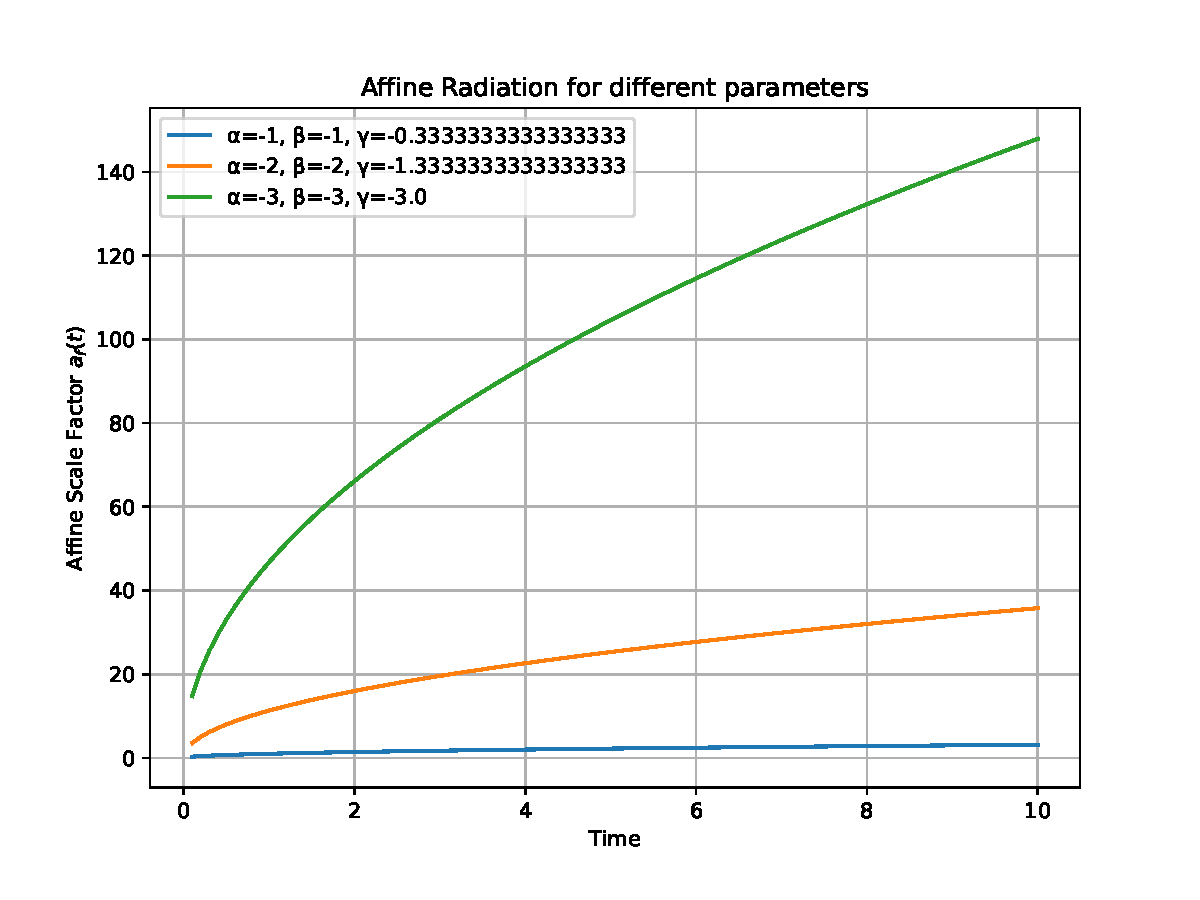
\includegraphics[scale=0.5]{Affine_Radiation}
%    \caption{Radiation era in PAG due to torsion effects}
%    \label{Affine_Radiation_plot}
%\end{figure}



In the same spirit, considering the case $\gamma = -\frac{2\alpha\beta}{5}$, leads to
\begin{equation}
    a_f(t) = a_{0}t^{2/3},
\end{equation}
where we defiend $a_0$ as 
\begin{equation}
    a_0 = \sqrt{-\alpha^{13/3}\beta^{10/3}}\left(\frac{2^{3/2}3^{2/3}}{5^{7/6}}\right)
\end{equation}    
which, in order to be real requires that $\beta <0$, which is consistent with constraint 
written in eq.\eqref{constraint}. This type of solution allow us to emulate a non-relativistic 
matter era.
%\begin{figure}[ht]
%    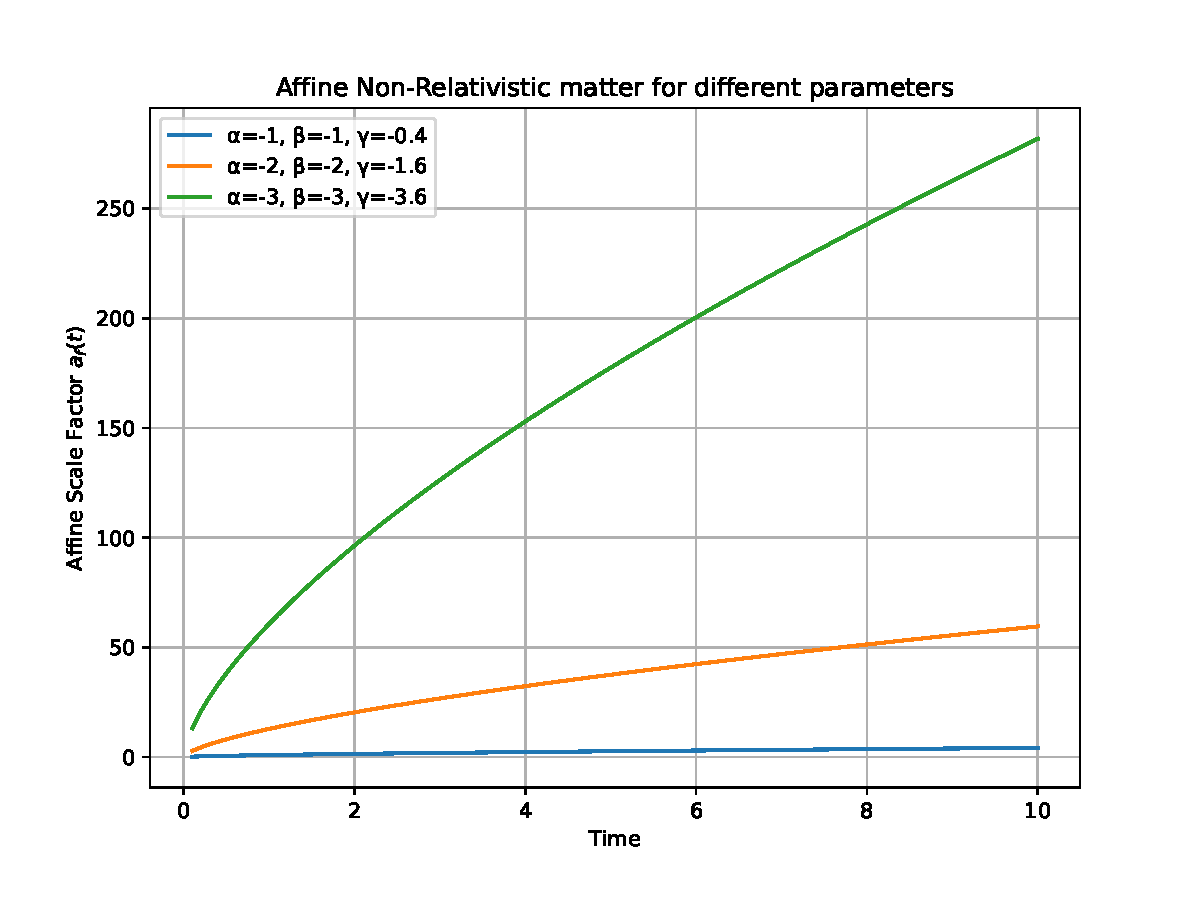
\includegraphics[scale=0.5]{Affine_Matter}
%    \caption{Non-relativistic matter era in PAG due to torsion effects}
%    \label{Affine_Matter_plot}
%\end{figure}
%A plot for different values of the parameters can be found in fig. \ref{Affine_Matter_plot}.

If we want to have an accelerated expansion due to torsion effects, we need to consider
\begin{equation}
    \label{acceleration_constraint}
    \ddot{a}_f > 0 \to \frac{\gamma\left(\alpha\beta + 2\gamma\right)}{\left(\alpha\beta + \gamma\right)^2}t^{\frac{\alpha\beta}{\alpha\beta + \gamma} - 3} > 0.
\end{equation}
the above condition, ensures a positive acceleration. In order to have a steady growth acceleration, it is required that 
\begin{equation}
    \label{restriction_acceleration}
    \alpha\beta < -\frac{3}{2}\gamma,
\end{equation}
this conditions ensures that the time evolution will be defined positive. Additionally, we have two branches coming from 
the numerator and denominator of eq. \eqref{acceleration_constraint}
\begin{align}
    B1: \alpha\beta & > -2\gamma & \gamma & > 0, \label{B1_a} \\
    B2: \alpha\beta & < -2\gamma & \gamma & < 0. \label{B2_a}
\end{align}
Using eq. \eqref{restriction_acceleration} along with eqs.\eqref{B1_a} and \eqref{B2_a} allow us to define to intervals for the
constant $\alpha\beta$, the former are $\alpha\beta \in \left[-2\gamma, -\frac{3}{2}\gamma\right]$, whereas the latter is given by $\alpha\beta <-2\gamma$. 
%\begin{figure}[ht]
%    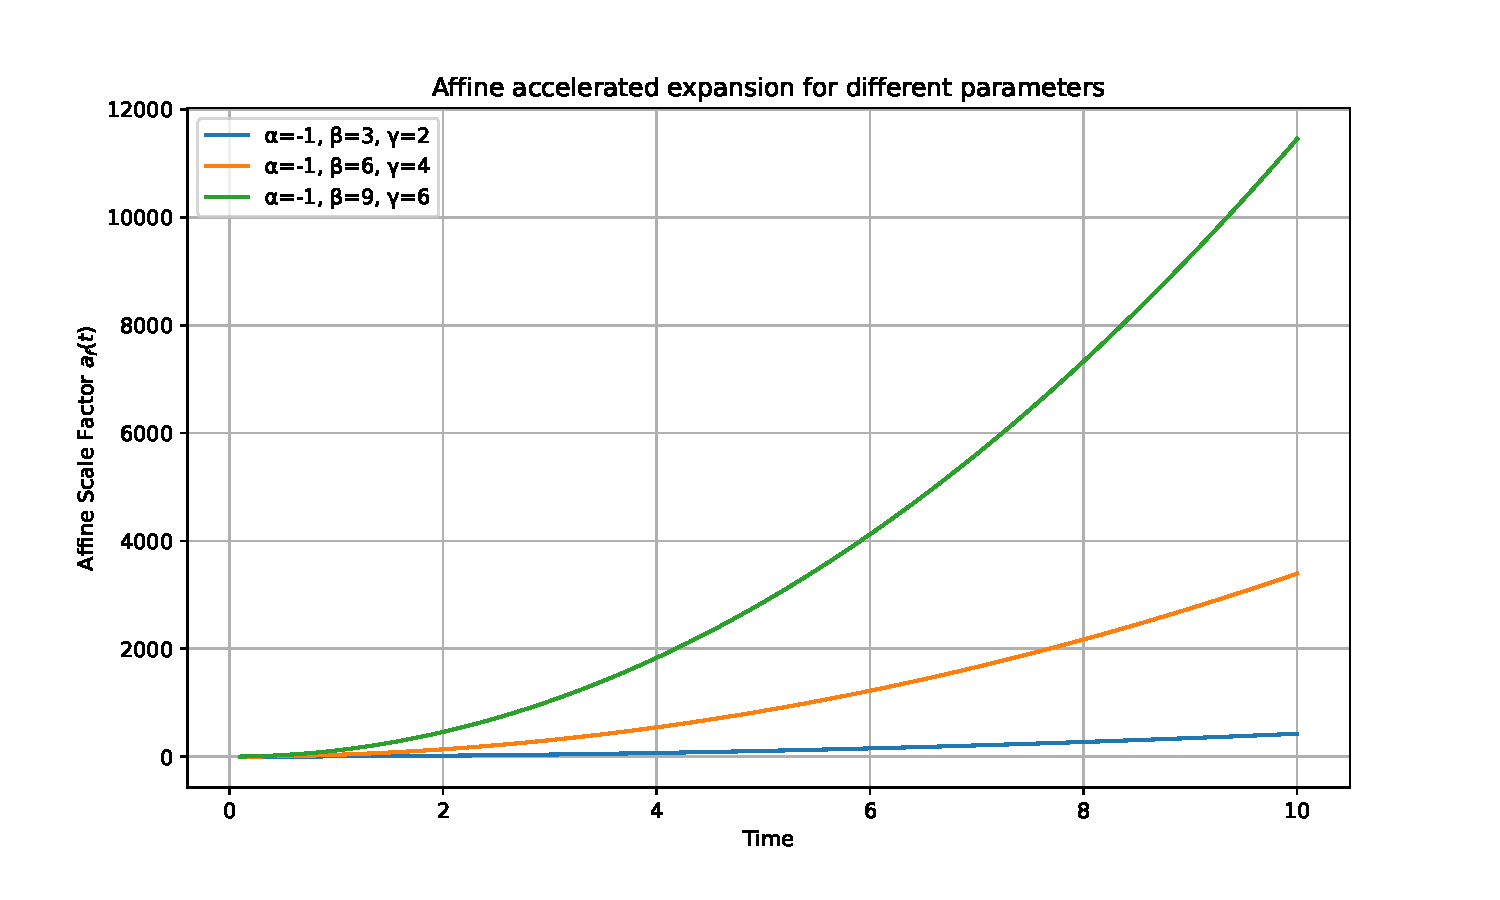
\includegraphics[scale=0.5]{Affine_Expansion}
%    \caption{Accelerated expansion in PAG due to torsion effects}
%    \label{Affine_Expansion_plot}
%\end{figure}
%A plot for different values of the parameters can be found in fig. \ref{Affine_Expansion_plot}.

\section{Final remarks}
\label{sec:final_remarks}

In this work, we have analyzed some cosmological scenarios appearing in the context of the Polynomial Affine Gravity model with torsion effects,
generalizing those considered in Refs.\cite{castillofelisola2019cosmological,Castillo_Felisola_2020}. Considering a non vanishing torsion tensor, 
yields an overdetermined system of differential equations, see eqs. \eqref{Feq_1} to \eqref{Feq_5}, unlike the case without torsion effects, whose
field equations are reduced to the \textit{harmonic curvature} $\nabla_\alpha \mathcal{R}_{\beta\gamma}{}^{\alpha}{}_{\delta} = 0$, which 
through Bianchi's identity can be written as an anti symmetrized covariant derivative of the Ricci tensor $\nabla_{[\mu} \mathcal{R}_{\alpha]\beta} = 0$.

Without torsion effects, the field equation leads to one differential equation for two unknown functions (see eq.\eqref{Feq_5} with $\eta(t) = 0$), thus,
the system can be solved parametrically, for example introducing an ansatz for $h(t)$ or $g(t)$. A priori, there is no physical
reason to fix one of the functions, however, one could explore subspace of this torsion-free solutions, by studying  integrability conditions
such as $\nabla_\alpha \mathcal{R}_{\beta\gamma} = 0$. This, leads to a three differential equations, which can be solved analytically 
and provides with an exact solution for $h(t)$ and $g(t)$ functions. Even more, the Ricci tensor is well behaved and it can be used 
as a metric tensor. This case yields well-known space lie de-Sitter/Anti de-Sitter solutions, where the cosmological constant is an
integration constant, see Ref.\cite{Castillo_Felisola_2020}.

The introduction of torsion fields with the tensors $\mathcal{B}$ and $\mathcal{A}$, induce 
nontrivial effects in the dynamics of the system. Due to the presence of the torsion tensor, 
there are two emergent descendent metric structures coming from the irreducible fields of the 
affine connection. Specifically, one comes from the symmetric part of the connection, which 
allow us to define the covariant derivative $\nabla^{\Gamma}$, and, the other one comes from 
the antisymmetric part of the affine connection, defined by the contraction of the product 
of two torsion tensors. 

Keeping in mind in the standard FLRW model of the universe, there are two fundamental objects, 
the metric tensor $g_{\mu\nu}$, and the energy-momentum tensor $T_{\mu\nu}$, we could argue
that in Polynomial Affine Gravity, the Ricci tensor $\mathcal{R}_{\mu\nu}$ can act as $g_{\mu\nu}$,
whereas $\mathcal{P}_{\mu\nu}$ emulate a $T_{\mu\nu}$. In that sense, the Ricci tensor provide us
an affine descendent scale factor, while the Poplawski like metric tensor emulate different types 
of matter effects,

Interestingly, the system of field equations eqs. \eqref{Feq_1} to \eqref{Feq_5} present four different 
branches of solution, of which only one can be solved exactly (non parametrically). This solution, has a 
nontrivial traceless part of the torsion $\psi(t)$, that resembles the energy density from General Relativity. 
Because of that, we considered different configurations of $\alpha$, $\beta$ and $\gamma$ parameters, 
and analyze their effects in the metric tensor coming from the Ricci. For specific values of those parameters, 
we were able to emulate the radiation era and the non-relativistic matter era. Additionally, we were able to 
define constraints for those parameters in order to secure an accelerated expansion, allowing us to emulate dark 
matter effects.

It has been sen that, the introduction of torsion effects in this affine model allow us to emulate matter
effects in the emergent metric structure coming from the Ricci tensor. In this formulation, the three major eras, are 
due to the presence of torsion and not an energy-momentum tensor. 

\section{Acknowledgments}

We are specially thankful to the developers and maintainers of SageMath \cite{sagemath}, SageManifolds 
\cite{Gourgoulhon_2015,Gourgoulhon_2018}, and Cadabra \cite{peeters2018introducing,Peeters2018,Peeters_2007}. Those softwares were 
used extensively in our calculations.

\bibliographystyle{unsrt}
\bibliography{References}

\end{document}